%%%%%%%%%%%%%%%%%%%%%%%%%%%%%%%%%%%%%%%%%%%%%%%%%%%%%%%%%%%%%%%%%%%%%%%%%%%%%%%%
% Copyright 2021 Louis Paternault --- http://ababsurdo.fr
%
% Publié sous licence Creative Commons Attribution-ShareAlike 4.0 International (CC BY-SA 4.0)
% http://creativecommons.org/licenses/by-sa/4.0/deed.fr
%%%%%%%%%%%%%%%%%%%%%%%%%%%%%%%%%%%%%%%%%%%%%%%%%%%%%%%%%%%%%%%%%%%%%%%%%%%%%%%%

% Compiler avec lualatex:
%$ lualatex $basename

\documentclass[12pt]{article}

\usepackage{2021-pablo}
\usepackage{2021-pablo-paternault}
\usepackage{2021-pablo-math}

\usepackage[
  a4paper,
  includehead,
  margin=10mm,
]{geometry}
\usepackage{2021-pablo-devoir}
\fancyhead[L]{\textsc{SNT > Internet > Protocole TCP-IP et Routage}}
\fancyhead[R]{\textsc{Corrigé}}

\renewcommand\thesubsection{\thesection.\alph{subsection}}

% Conversion des nombres en lettres
\makeatletter
\newcommand{\makeAlph}[1]{\@Alph{#1}}
\makeatother

\usepackage{2021-pablo-tikz}

\begin{document}

Corrigé de l'activité : \url{https://snt.ababsurdo.fr/internet/tcp-ip/}.

\section{Tous et toutes connectées}
\subsection{Réseau centralisé}

\begin{enumerate}
  \item Voici le schéma à neuf ordinateurs : l'ordinateur $A$ est central, et chacun des autres est relié à lui.
    \begin{center}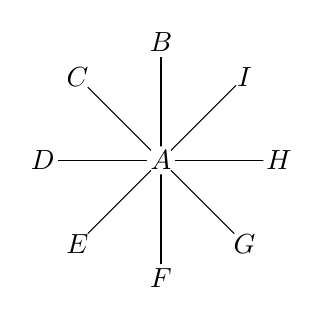
\begin{tikzpicture}[scale=1.5]
        \tikzstyle{sommet}=[circle, fill=white, minimum size=0em, inner sep=0];

        \coordinate (A) at (0, 0);

        \foreach \i in {2,..., 9}{
          \coordinate (A\i) at ({360/8*\i}:1);
          \draw (A) -- (A\i);
          \draw (A\i) node[sommet]{$\makeAlph{\i}$};
        }
        \draw (A) node[sommet]{$A$};
    \end{tikzpicture}\end{center}
  \item Il faut huit câbles pour réaliser cette configuration.
\end{enumerate}

\subsection{Réseau décentralisé}
\begin{center}\begin{tikzpicture}
    \tikzstyle{sommet}=[circle, fill=white, minimum size=0em, inner sep=0];

    \coordinate (A) at (0, 0);
    \coordinate (B) at (0:1);
    \coordinate (C) at (120:1);
    \coordinate (D) at (240:1);
    \begin{scope}[shift={($1.5*(B)$)}]
      \coordinate (E) at (-60:.5);
      \coordinate (F) at (60:.5);
    \end{scope}
    \begin{scope}[shift={($1.5*(C)$)}]
      \coordinate (G) at (60:.5);
      \coordinate (H) at (180:.5);
    \end{scope}
    \begin{scope}[shift={($1.5*(D)$)}]
      \coordinate (I) at (240:.5);
    %\coordinate (J) at (300:.5);
    \end{scope}

    \draw (I) -- (D) -- (A) -- (B) -- (E);
    \draw (B) -- (F);
    \draw (H) -- (C) -- (G);
    \draw (A) -- (C);
    \draw (A) node[sommet]{$A$};
    \draw (B) node[sommet]{$B$};
    \draw (C) node[sommet]{$C$};
    \draw (D) node[sommet]{$D$};
    \draw (E) node[sommet]{$E$};
    \draw (F) node[sommet]{$F$};
    \draw (G) node[sommet]{$G$};
    \draw (H) node[sommet]{$H$};
    \draw (I) node[sommet]{$I$};
\end{tikzpicture}\end{center}
\begin{enumerate}
  \item Il faut aussi huit câbles pour réaliser cette configuration.
  \item Quel que soit le câble coupé, un ou plusieurs ordinateurs seront exclus du réseau.
  \item
    \begin{enumerate}
      \item Un message allant de $E$ à $C$ passe par les ordineateurs $B$ et $A$.
      \item Un message allant de $G$ à $H$ passe par l'ordinateur $C$.
      \item Toutes les communications ne passent donc pas par le même ordinateur, même si l'ordinateur $A$ a toujours une place importante dans le réseau : \emph{beaucoup} de configurations passent par lui.
    \end{enumerate}
  \item 
    \begin{enumerate}
      \item Si un des ordinateurs $A$, $B$, $C$, $D$ tombe en panne, d'autres ordinateurs ne peuvent plus communiquer.
      \item Si l'ordinateur $F$ (par exemple) tombe en panne, les autres ordinateurs peuvent continuer à communiquer comme si de rien n'était.
    \end{enumerate}
\end{enumerate}
\subsection{Graphe complet}

\begin{enumerate}
  \item Voici la configuration à neuf ordinateur, où chacun d'entre eux est relié directement à chacun des autres.
    \begin{center}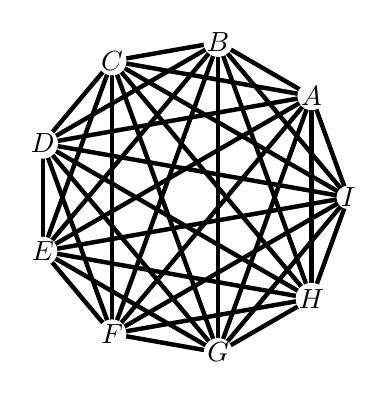
\begin{tikzpicture}[scale=2, ultra thick]
        \tikzstyle{sommet}=[circle, fill=white, minimum size=0em, inner sep=0];

        \foreach \i in {1,..., 9}{
          \coordinate (A\i) at ({360/9*\i}:1);
          \foreach \j in {1, ..., \i}{
            \draw (A\i) -- (A\j);
          }
        }
        \foreach \i in {1,..., 9}{
          \draw (A\i) node[sommet]{$\makeAlph{\i}$};
        }
    \end{tikzpicture}\end{center}
  \item Il est nécessaire d'utiliser 36 câbles. On peut soit compter les arêtes sur le schéma ci-dessus, soit raisonner comme suit.

    Puisque chacun des 9 ordinateurs est relié aux 8 autres, cela fait $9\times8=72$ câbles. Mais en comptant ainsi, on a compté à la fois le câble allant de $A$ à $B$, et celui allant de $B$ à $A$, alors que c'est le même câble, et de même pour les autres couples d'ordinateurs. Chacun des câbles a donc été compté deux fois. Il faut donc diviser ce nombre par deux pour trouver le bon nombre de câbles : $72\div2=36$.
  \item Pour aller de $A$ à $B$, il est possible de passer par $C$, ou par $D$, ou par $I$ puis $J$ puis $H$, ou\ldots
  \item Aucun ordinateur ne contrôle l'ensemble des communications ; aucun ordinateur ne contrôle donc le réseau plus que les autres.
  \item De même, aucun ordinateur n'a une plus importante que d'autres dans ce réseau, et chacun des ordinateurs peut tomber en panne sans perturber les communications.
\end{enumerate}

\subsection{Réseau acentré}

\begin{center}
  \begin{tikzpicture}
    \tikzstyle{sommet}=[circle, fill=white, minimum size=0em, inner sep=0];

    \coordinate (A) at (0:1);
    \coordinate (D) at (120:1);
    \coordinate (G) at (240:1);
    \begin{scope}[shift={($1.5*(A)$)}]
      \coordinate (B) at (-60:.5);
      \coordinate (C) at (60:.5);
    \end{scope}
    \begin{scope}[shift={($1.5*(D)$)}]
      \coordinate (E) at (60:.5);
      \coordinate (F) at (180:.5);
    \end{scope}
    \begin{scope}[shift={($1.5*(G)$)}]
      \coordinate (H) at (180:.5);
      \coordinate (I) at (300:.5);
    \end{scope}

    \draw (A) -- (B) -- (C) -- (A) -- (D) -- (E) -- (F) -- (D) -- (G) -- (H) -- (I) -- (G) -- cycle;
    \draw (A) node[sommet]{$A$};
    \draw (B) node[sommet]{$B$};
    \draw (C) node[sommet]{$C$};
    \draw (D) node[sommet]{$D$};
    \draw (E) node[sommet]{$E$};
    \draw (F) node[sommet]{$F$};
    \draw (G) node[sommet]{$G$};
    \draw (H) node[sommet]{$H$};
    \draw (I) node[sommet]{$I$};
  \end{tikzpicture}
\end{center}

\begin{enumerate}
  \item On compte 12 câbles sur ce réseau, ce qui est supérieur à la configuration de départ (tous les ordinateurs reliés à $A$), mais bien inférieur à la configuration de départ (où chacun des ordinateurs était relié à chacun des autres).
  \item On peut suivre le chemin $B-C-A-G-D-F$.
  \item Aucun ordinateur ne contrôle toutes les communications.
  \item Certains ordinateurs, s'ils tombent en panne, coupent le réseau ($A$, $D$, $G$ ici), mais d'autres non.
\end{enumerate}

\subsection{Bilan}
\emph{Aucune question.}
\section{IP, un protocole universel ?}
\emph{QCM corrigé sur Pronote.}

\end{document}
